%%%
%
% $Autor: Wings $
% $Datum: 2021-05-14 $
% $Pfad: GitLab/CornerBLending $
% $Dateiname: Hints
% $Version: 4620 $
%
% !TeX spellcheck = de_DE/GB
%
%%%



\chapter{Hints}

Please, use  \textbf{\texttt{biber.exe}}.

\bigskip

If you want to create a symbol directory, call makeindex:


\textbf{\texttt{makeindex \%.nlo -s nomencl.ist}}


\section{Added by Sadegh (To be deleted at the end of the project)}

Don't use numbers 1, 2, ... for your files(images, code, etc.)

There should be subfolders in the images directory. 

\section{Sample section}

This is a sample section

\subsection{Sample subsection}

This is a subsection.

\subsubsection{Sample subsubsection}

This is a subsubsection.


\section{Itemize and enumerate}

\begin{itemize}
	\item Item 1
	\item Item 2
	\item Item 3
\end{itemize}

\begin{enumerate}
	\item First item
	\item Second item
	\item Third item
\end{enumerate}


\section{Text Formatting (Bold, Italic, ...)}

\textbf{This is bold text.}

\emph{This is italicized text.}

\texttt{This is monospace (typewriter) text.}

To define a Python function, variable, class, etc. use : 

The \PYTHON{print()} function does ...

To define other objects that are not in Python you can use \texttt{\textbackslash texttt}

Here is some \texttt{monospaced text} for example.

to add a url:

Example: Download the Windows installer for Doxygen from the official website: \url{https://www.doxygen.nl/download.html}.


\section{Font Sizes}

\textbf{Note:} only change if necessary!

{\tiny This is tiny text.}

{\scriptsize This is scriptsize text.}

{\footnotesize This is footnotesize text.}

{\small This is small text.}

{\normalsize This is normal text.}

{\large This is large text.}

{\Large This is Large text.}

{\LARGE This is LARGE text.}

{\huge This is huge text.}

{\Huge This is Huge text.}


\section{Tables, figures, code, and equations}

Notice the caption, and label. Always use label and refer to your figures and tables in the text using \texttt{\textbackslash ref}. Also notice the convention we use in labeling each one. For example for figures, we use \texttt{fig:sampleLabel}.

In the Figure \ref{fig:sampleLabel} 

\begin{figure}[h!]
	\centering
	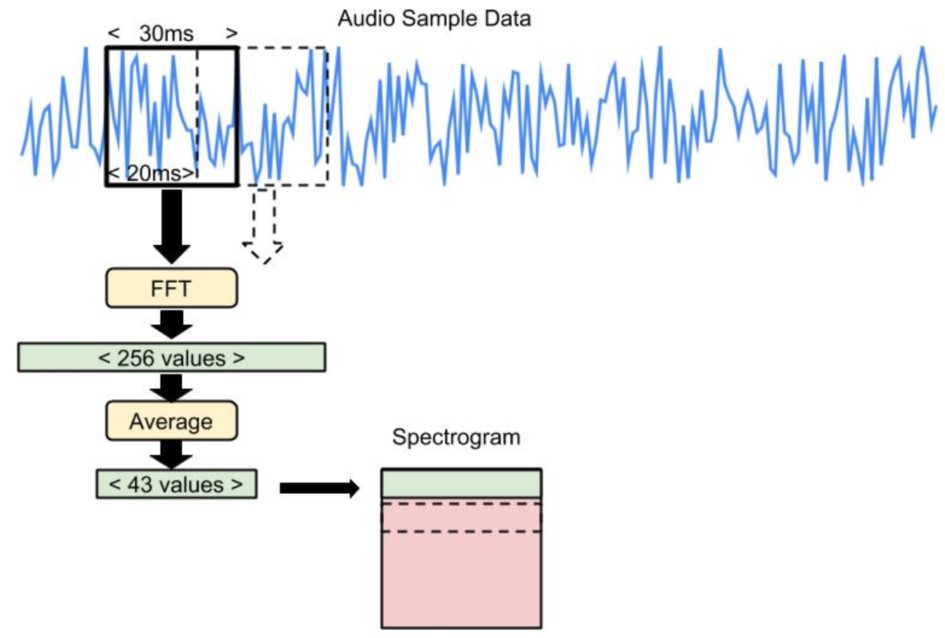
\includegraphics[width=0.8\textwidth]{Images/DataMining/audioProcessing.jpg}
	\caption{Diagram of the processing of audio samples \cite{Warden:2019}.} \label{fig:audioProcessing}
\end{figure}
Your text (see Listing \ref{code:sampleCode})

\begin{code}[h!]
	\lstinputlisting[language=Python, numbers=none, linerange={99-114}]{Code/DoxygenManual/DoxygenManual.py}    
	
	\caption{Sample code}
	\label{code:sampleCode}
\end{code}

As shown in the Table \ref{table:modelEvaluation}

\begin{table}[h!]
	\footnotesize
	\centering
	\caption{Model Evaluation Metrics}\label{table:modelEvaluation}
	\begin{tabular}{lcccc}
		\hline
		Model                               & $R^2$ (Train) & $\text{R}^2$ (Test) & MSE (Train) & MSE (Test)    \\ \hline
		Linear Regression                   & 0.53      & 0.45         & 2.87e+03 & 2900.19  \\ 
		Polynomial Regression (degree=4)    & 1.00      & -26.73       & 9.79e-23 & 1.47e+05  \\ 
		Ridge Regression                    & 0.52      & 0.46         & 2.90e+03 & 2865.18  \\ 
		Lasso Regression                    & 0.50      & 0.47         & 3.03e+03 & 2809.50  \\ 
		Elastic Net Regression              & 0.14      & 0.13         & 5.25e+03 & 4605.03  \\ 
		Decision Tree Regression            & 1.00      & 0.06         & 0.00     & 4976.80  \\ 
		Support Vector Regression           & 0.17      & 0.18         & 5.06e+03 & 4332.74  \\ 
		\hline
	\end{tabular}
\end{table}


The required parameters in equation \ref{eq:parametersEstimate} are calculated by minimizing the equation \ref{eq:RSSlinear}, Where $n$ is the total number of data points, $y_i$ represents the actual observed value of the dependent variable for the ith data point. RSS is the Residual Sum of Squares.

\begin{equation}\label{eq:parametersEstimate}
	\text{parameters to estimate: }
	\left\{
	\begin{aligned}
		\boldsymbol{\hat{w}} & = (\hat{w}_0, \hat{w}_1, \ldots, \hat{w}_n) \text{: feature weights}\\
		\boldsymbol{\hat{b}} & = \text{intercept term}
	\end{aligned}
	\right.
\end{equation}

\begin{equation}\label{eq:RSSlinear}
	\text{RSS}_{linear} (\boldsymbol{\hat{w}}, \boldsymbol{\hat{b}}) = \sum_{i=1}^{n} (\boldsymbol{y_i} - (\boldsymbol{\hat{w}} x_i + \boldsymbol{\hat{b}}))^2
\end{equation}


\section{Citations (References)}

This is the directory of the citations file: ML23-01-Keyword-Spotting-with-an-Arduino-Nano-33-BLE-Sense/Literature/MyLiterature.bib

All the downloadable literature should be downloaded and pushed to GitHub. This is an example to show how to cite:

Automatic speech recognition in digital assistants has become a prominent application of artificial neural networks in the consumer space \cite{Bushur:2023}.

For citing a document:

\begin{enumerate}
	\item Go to the \url{https://scholar.google.com/} and find the appropriate article or book.
	
	\begin{itemize}
		\item \textbf{Note:} Do not use websites as references unless there's no way out of it!!!
	\end{itemize}
	
	\item Under the article title click on \texttt{Cite} and then clicle on \texttt{BibTeX}.
	\item Copy the content and paste it in the \texttt{MyLiterature.bib} file and save it (open the file with notepad or notpad+++ etc.). Remember to follow the style in the .bib file. Remember to manually add the \textbf{doi} (if it's an article) or \textbf{isbn} (if it's a book) in the last line
	
	\begin{itemize}
		\item The directory of the .bib file is \texttt{ML23-01-Keyword-Spotting-with-an-Arduino-Nano-33-BLE-Sense/Documents}
	\end{itemize}
	
	\item Use the \texttt{cite{}} command in the report.
	\item Download the PDF file of that article (if there is a possibility of downloading) and move it to the directory \texttt{ML23-01-Keyword-Spotting-with-an-Arduino-Nano-33-BLE-Sense/Documents/Literature}
\end{enumerate}

If the citation is not showing in the report, there might be a problem in the latex files, don't panic!!!
